\documentclass{article}
\usepackage{graphicx}
\usepackage{amsmath,amssymb,amsthm}
\usepackage{float}
\usepackage{array}


\title{Convolution}
\author{Gunda Srihaas}
\date{}

\begin{document}

\maketitle

\section{Question} 
Compute the convolution of a given signal f(t) with a rectangular kernel h(t), analytically. The rectangular kernel
is defined as:
\[
h(t)=
\begin{cases}
    1, & \text{for } -T \leq t \leq T \\
    0, & \text{otherwise}
\end{cases}
\]
Derive the convolution expression $y(t) = (f * h)(t)$ in terms of known functions, and analyze the system’s behavior
for various values of the kernel duration T and the input signal $f(t)$. Additionally, investigate the following scenarios:\\
\begin{enumerate}
\item[a.] Modify the kernel to only consider the part of the kernel for $t > 0$. How does this affect the convolution result?\\
\item [b.] Shift the kernel by a time $\tau_0$. Analyze how the shift impacts the convolution output and discuss the significance
of this shift in the context of time-delayed systems
\end{enumerate}

\section{Solution}
\subsection{\textbf{Taking $f(t)= sin(\omega t)$}}
The convolution is defined as:
\begin{align*}
y(t) = (f * h)(t) = \int_{-\infty}^{\infty} f(\tau) h(t - \tau) \, d\tau
\end{align*}

Given,
\begin{align*}
h(t)=
\begin{cases}
    1, & \text{for } -T \leq t \leq T \\
    0, & \text{otherwise}
\end{cases}
\end{align*}

Which implies in convolution,
\begin{align*}
    -T \leq t - \tau \leq T \\
    t-T \leq \tau \leq t+T
\end{align*}

$\implies h(t-\tau)=1$ in $(t-T,t+T)$
\\
Thus, the convolution integral becomes:
\begin{align*}
y(t) = \int_{t - T}^{t + T} f(\tau) \, d\tau
\end{align*}

For $f(t) = \sin(\omega t)$, the convolution becomes:
\[
y(t) = \int_{t - T}^{t + T} \sin(\omega \tau) \, d\tau
\]

\begin{align*}
y(t) &= \int_{t - T}^{t + T} \sin(\omega \tau) \, d\tau \\
&= \left[ -\frac{1}{\omega} \cos(\omega \tau) \right]_{t - T}^{t + T} \\
&= -\frac{1}{\omega} \left[ \cos(\omega (t + T)) - \cos(\omega (t - T)) \right]
\end{align*}

Using the trigonometric identity:
\begin{align*}
\cos A - \cos B = -2 \sin\left(\frac{A + B}{2}\right) \sin\left(\frac{A - B}{2}\right) \end{align*}

Let:
\begin{align*}
A &= \omega (t + T) \\
B &= \omega (t - T)
\end{align*}

Then:
\begin{align*}
\frac{A + B}{2} &= \omega t \\
\frac{A - B}{2} &= \omega T
\end{align*}

Substituting:
\begin{align*}
y(t) &= -\frac{1}{\omega} \left[ -2 \sin(\omega t) \sin(\omega T) \right] \\
&= \frac{2}{\omega} \sin(\omega T) \sin(\omega t)
\end{align*}

\textbf{Final Result}
\begin{align*}
y(t) = \frac{2}{\omega} \sin(\omega T) \sin(\omega t)    
\end{align*}
\newpage
\subsection{Taking any periodic $f(t)$}
\begin{align*}
f(t) = A_0 + \sum_{n=1}^\infty A_n \cos\left(\frac{n\pi t}{L}\right) + \sum_{n=1}^\infty B_n \sin\left(\frac{n\pi t}{L}\right)
\end{align*}
By substitution of $f(t)$ and and reducing the integral we get
\begin{align*}
y(t) = \int_{t - T/2}^{t + T/2} \left[ A_0 + \sum_{n=1}^\infty A_n \cos\left(\frac{n\pi \tau}{L}\right) + \sum_{n=1}^\infty B_n \sin\left(\frac{n\pi \tau}{L}\right) \right] d\tau
\end{align*}
\\
\textbf{DC Term}
\begin{align*}
\int_{t - T/2}^{t + T/2} A_0 \, d\tau = A_0 T
\end{align*}
\\
\paragraph{Sine part}
\begin{align*}
B_n \int \sin\left(\frac{n\pi \tau}{L}\right) d\tau = -\frac{L}{n\pi} \cos\left(\frac{n\pi \tau}{L}\right)
\end{align*}
Evaluating from $t - T/2$ to $t + T/2$:
\begin{align*}
B_n \cdot \frac{2L}{n\pi} \cos\left(\frac{n\pi t}{L}\right) \sin\left(\frac{n\pi T}{2L}\right)
\end{align*}
\\
\textbf{Cosine part}
\begin{align*}
y_{\text{cos}}(t) &= \int_{t - T}^{t + T} A_n \cos\left(\frac{n\pi \tau}{L}\right) \, d\tau \\
&= A_n \left[ \frac{L}{n\pi} \sin\left(\frac{n\pi \tau}{L}\right) \right]_{t - T}^{t + T} \\
&= A_n \cdot \frac{L}{n\pi} \left[ \sin\left(\frac{n\pi (t + T)}{L}\right) - \sin\left(\frac{n\pi (t - T)}{L}\right) \right]
\end{align*}

Using the trigonometric identity:
\begin{align*}
\sin C - \sin D = 2 \cos\left(\frac{C + D}{2}\right) \sin\left(\frac{C - D}{2}\right)
\end{align*}

Let:
\begin{align*}
C &= \frac{n\pi (t + T)}{L} = \frac{n\pi t}{L} + \frac{n\pi T}{L} \\
D &= \frac{n\pi (t - T)}{L} = \frac{n\pi t}{L} - \frac{n\pi T}{L}
\end{align*}

Then:
\begin{align*}
\frac{C + D}{2} &= \frac{n\pi t}{L} \\
\frac{C - D}{2} &= \frac{n\pi T}{L}
\end{align*}

Substituting:
\begin{align*}
y_{\text{cos}}(t) &= A_n \cdot \frac{L}{n\pi} \left[ 2 \cos\left(\frac{n\pi t}{L}\right) \sin\left(\frac{n\pi T}{L}\right) \right] \\
&= A_n \cdot \frac{2L}{n\pi} \sin\left(\frac{n\pi T}{L}\right) \cos\left(\frac{n\pi t}{L}\right)
\end{align*}

\subsection*{Final Result}
\begin{align*}
y(t) = 2A_0 T + \sum_{n=1}^\infty \frac{2L}{n\pi} \sin\left(\frac{n\pi T}{L}\right) \left[ A_n \sin\left(\frac{n\pi t}{L}\right) + B_n \cos\left(\frac{n\pi t}{L}\right) \right]
\end{align*}

\section*{Convolution of a Signal with a Rectangular Kernel}

Given a signal $f(t)$ and a rectangular kernel $h(t)$ defined as:
\[
h(t)=
\begin{cases}
    1, & \text{for } -T \leq t \leq T \\
    0, & \text{otherwise}
\end{cases}
\]
The convolution $y(t) = (f * h)(t)$ is:
\begin{align*}
y(t) = \int_{-\infty}^{\infty} f(\tau) h(t - \tau) \,d\tau
\end{align*}

\subsection*{Part 1: General Convolution Expression}
The kernel $h(t - \tau)$ is 1 when $-T \leq t - \tau \leq T$, i.e., $t - T \leq \tau \leq t + T$. Thus:
\begin{align*}
y(t) = \int_{t - T}^{t + T} f(\tau) \,d\tau
\end{align*}

\subsection*{Part 2: Analysis for Various $T$ and $f(t)$}
\begin{itemize}
    \item \textbf{Large $T$:} More smoothing of $f(t)$, attenuates high frequencies.
    \item \textbf{Small $T$:} Less smoothing, $y(t) \approx f(t)$.
    \item \textbf{Constant $f(t) = c$:} $y(t) = 2T c$.
    \item \textbf{Linear $f(t) = a t + b$:} 
    \begin{align*}
    y(t) &= \int_{t - T}^{t + T} (a \tau + b) \,d\tau \\
         &= 2a T t + 2T b
    \end{align*}
\end{itemize}

\subsection*{Part a: Modified Kernel ($t > 0$)}
Define:
\[
h_{\text{modified}}(t)=
\begin{cases}
    1, & \text{for } 0 \leq t \leq T \\
    0, & \text{otherwise}
\end{cases}
\]
The convolution becomes:
\begin{align*}
y_{\text{modified}}(t) = \int_{t - T}^{t} f(\tau) \,d\tau
\end{align*}
\textbf{Difference:}
\begin{itemize}
    \item Original: Integrates symmetrically around $t$ ($[t - T, t + T]$).
    \item Modified: Only integrates past values ($[t - T, t]$), making it causal.
\end{itemize}

\subsection*{Part b: Shifted Kernel by $\tau_0$}
Shifted kernel:
\[
h_{\text{shifted}}(t) = h(t - \tau_0) =
\begin{cases}
    1, & \text{for } \tau_0 - T \leq t \leq \tau_0 + T \\
    0, & \text{otherwise}
\end{cases}
\]
The convolution is:
\begin{align*}
y_{\text{shifted}}(t) &= \int_{t - \tau_0 - T}^{t - \tau_0 + T} f(\tau) \,d\tau \\
                      &= y(t - \tau_0)
\end{align*}
\textbf{Interpretation:} Shifting the kernel by $\tau_0$ shifts the output by $\tau_0$.

\subsection*{Specific Cases for $f(t)$}
\subsubsection*{Case 1: $f(t) = \sin(\omega t)$}
\begin{align*}
y(t) &= \int_{t - T}^{t + T} \sin(\omega \tau) \,d\tau \\
     &= \frac{2 \sin(\omega T)}{\omega} \sin(\omega t)
\end{align*}
For shifted kernel:
\begin{align*}
y_{\text{shifted}}(t) = \frac{2 \sin(\omega T)}{\omega} \sin(\omega (t - \tau_0))
\end{align*}

\subsubsection*{Case 2: Fourier Series Representation}
Let:
\begin{align*}
f(t) = A_0 + \sum_{n=1}^\infty A_n \cos\left(\frac{n\pi t}{L}\right) + \sum_{n=1}^\infty B_n \sin\left(\frac{n\pi t}{L}\right)
\end{align*}
Then:
\begin{align*}
y(t) &= 2 T A_0 + \sum_{n=1}^\infty \frac{2 L}{n \pi} \sin\left(\frac{n \pi T}{L}\right) \left[ A_n \cos\left(\frac{n \pi t}{L}\right) + B_n \sin\left(\frac{n \pi t}{L}\right) \right]
\end{align*}
For shifted kernel:
\begin{align*}
y_{\text{shifted}}(t) &= 2 T A_0 + \sum_{n=1}^\infty \frac{2 L}{n \pi} \sin\left(\frac{n \pi T}{L}\right) \\
&\quad \times \left[ A_n \cos\left(\frac{n \pi (t - \tau_0)}{L}\right) + B_n \sin\left(\frac{n \pi (t - \tau_0)}{L}\right) \right]
\end{align*}

\begin{figure}[H]
    \centering
    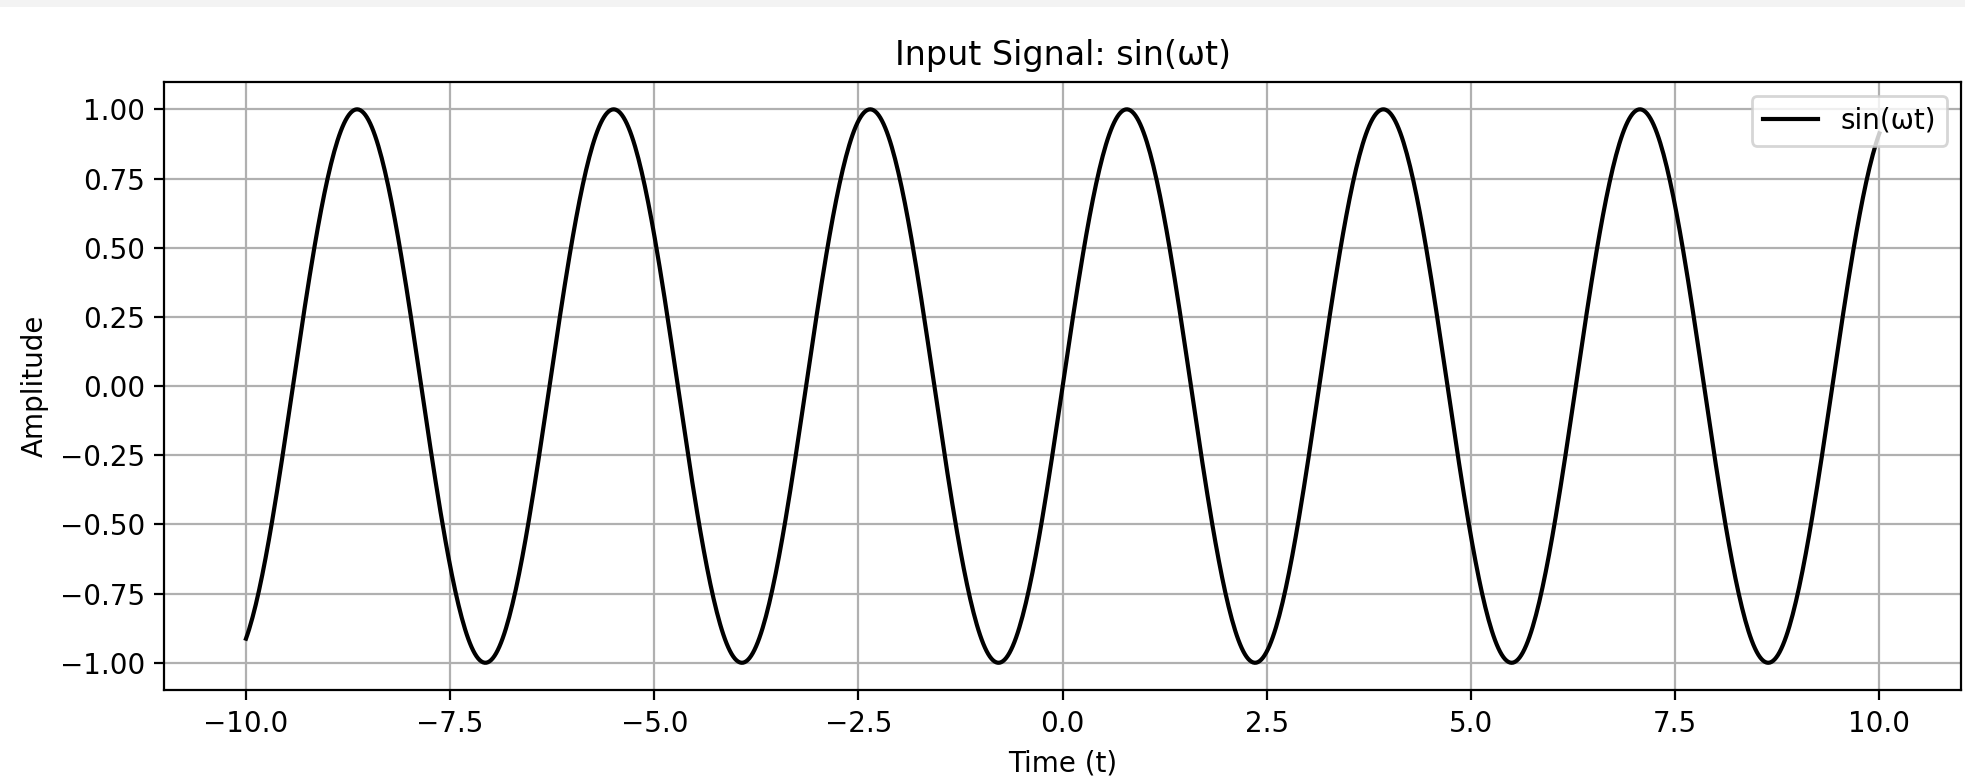
\includegraphics[width=\linewidth]{figs/sinwt.png}
\end{figure}
\begin{figure}[H]
    \centering
    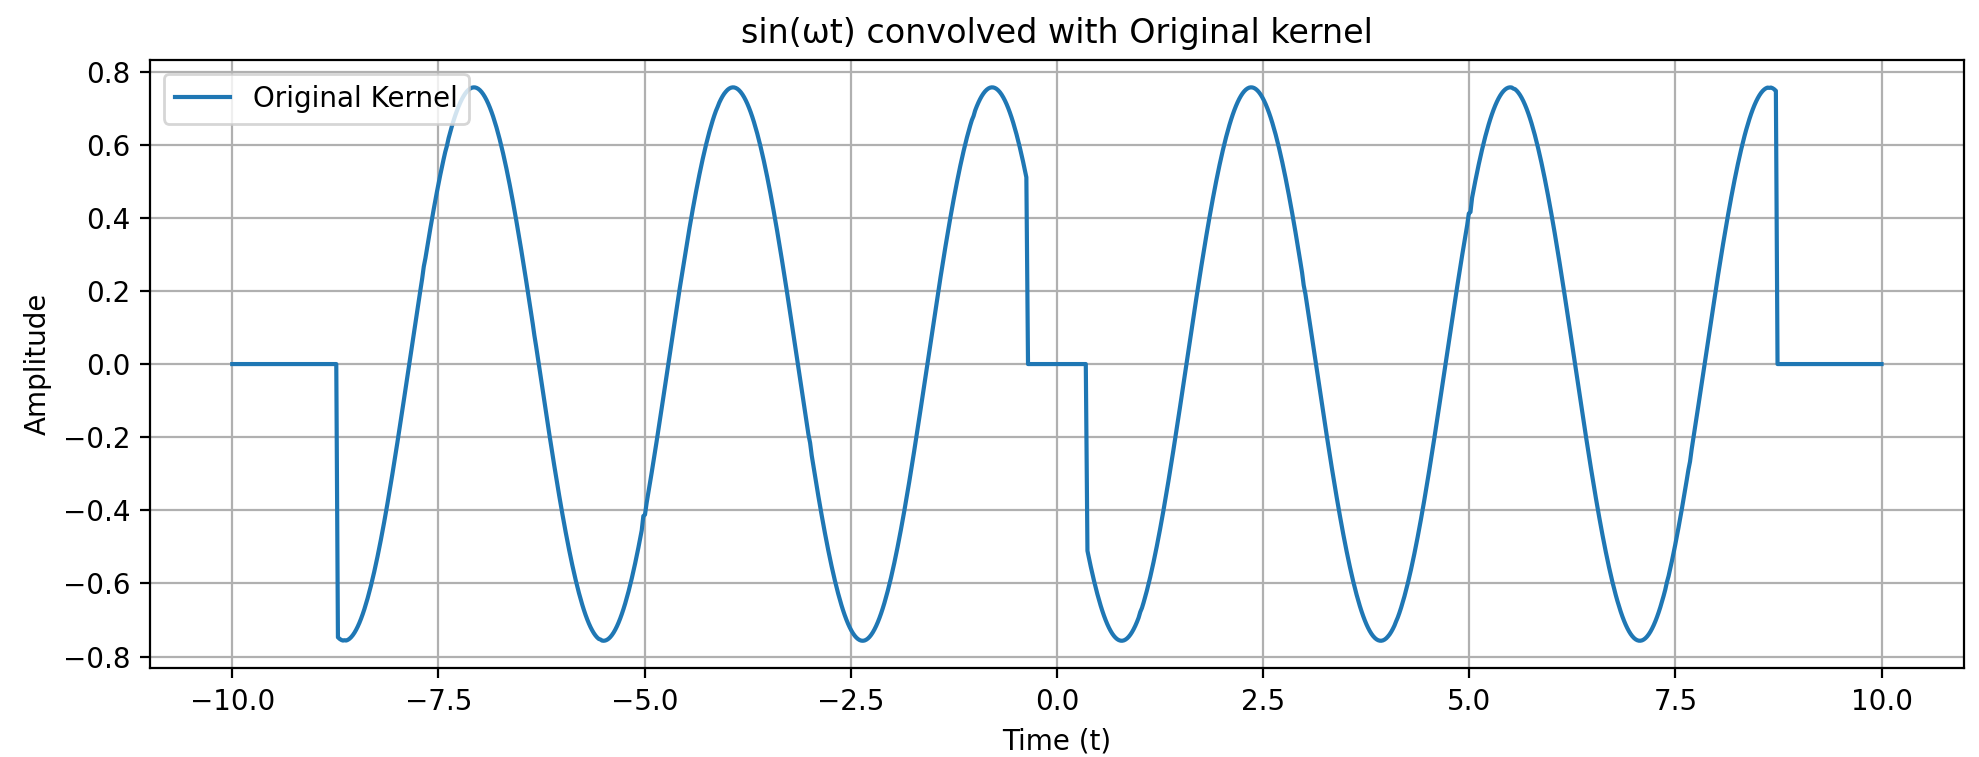
\includegraphics[width=\linewidth]{figs/sinconv.png}
\end{figure}
\newpage
\begin{figure}[H]
    \centering
    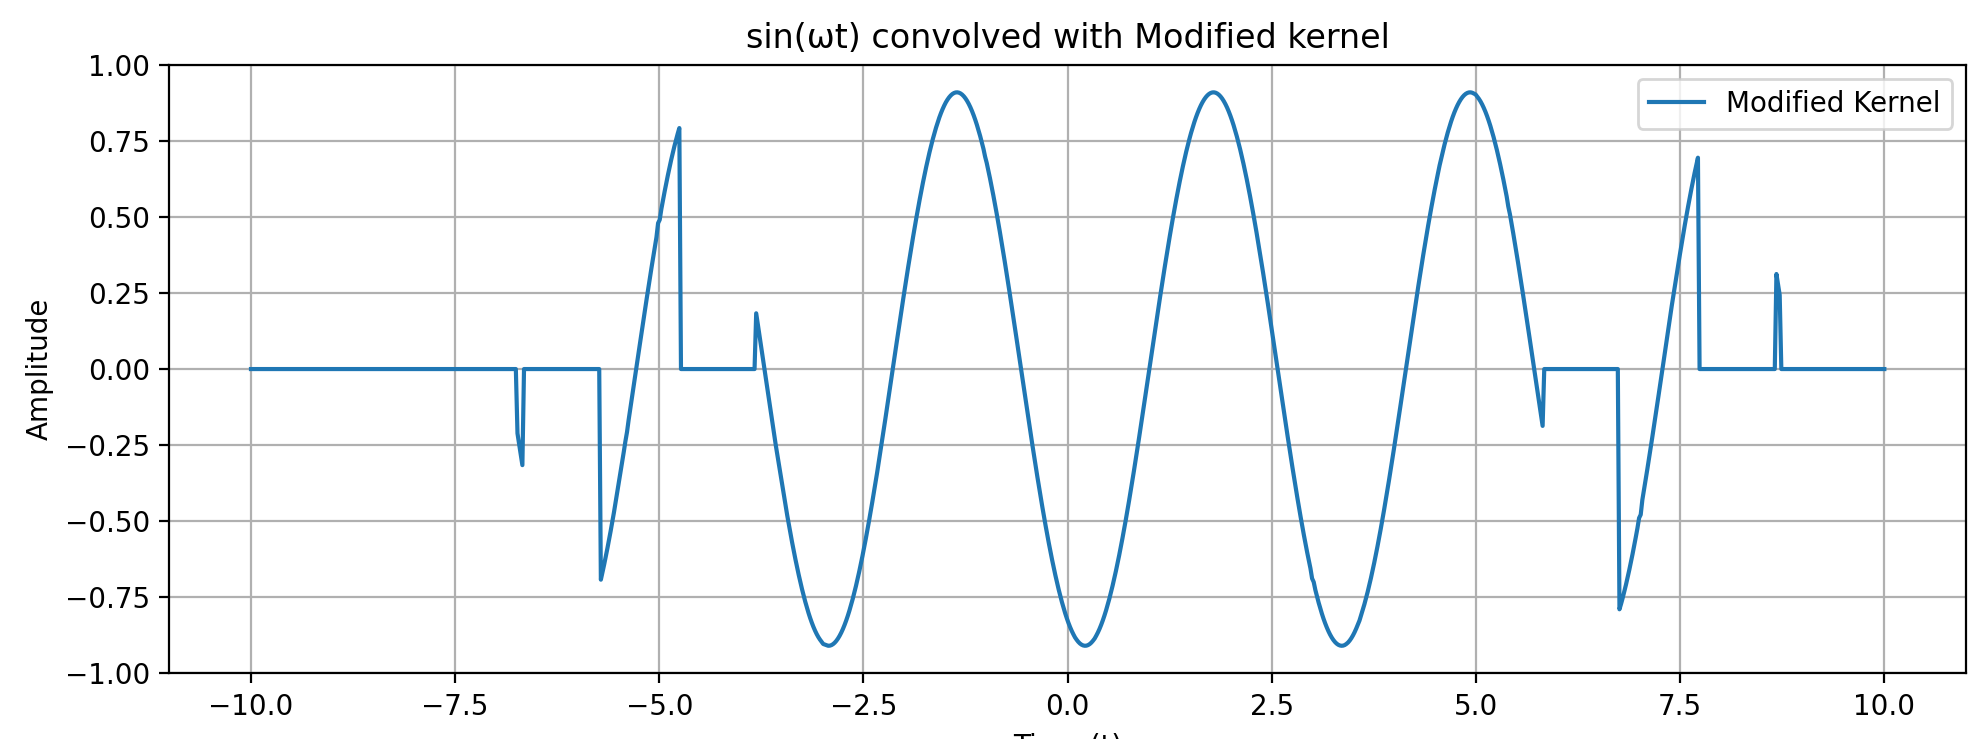
\includegraphics[width=\linewidth]{figs/modifiedsin.png}
\end{figure}
\begin{figure}[H]
    \centering
    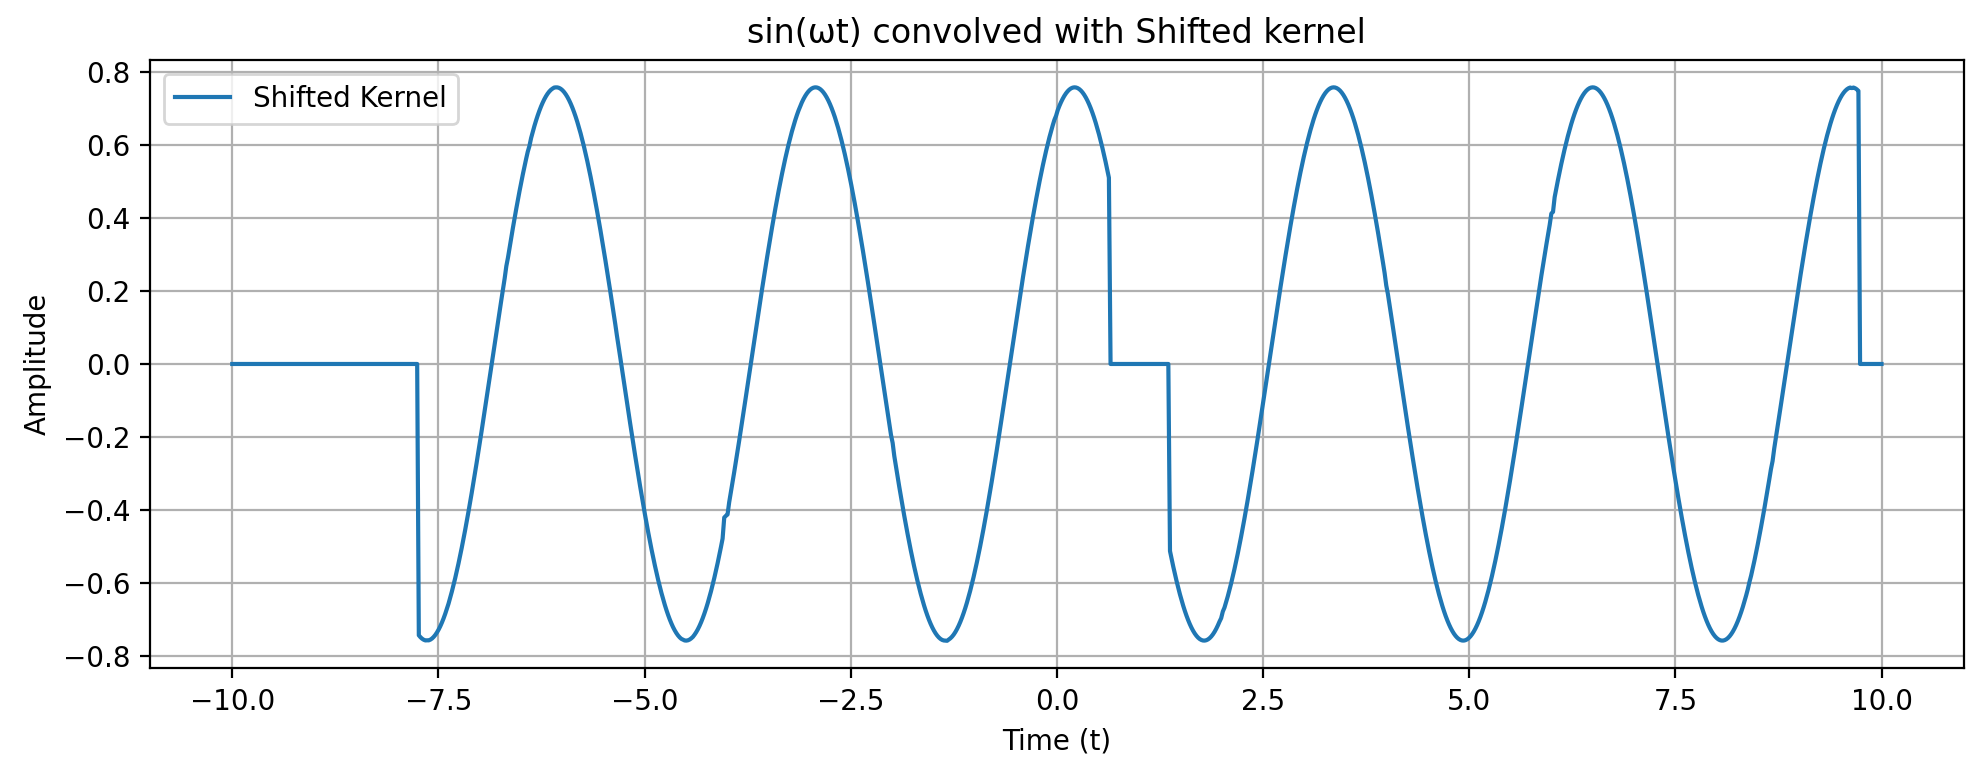
\includegraphics[width=\linewidth]{figs/shiftedsin.png}
\end{figure}

\begin{figure}[H]
    \centering
    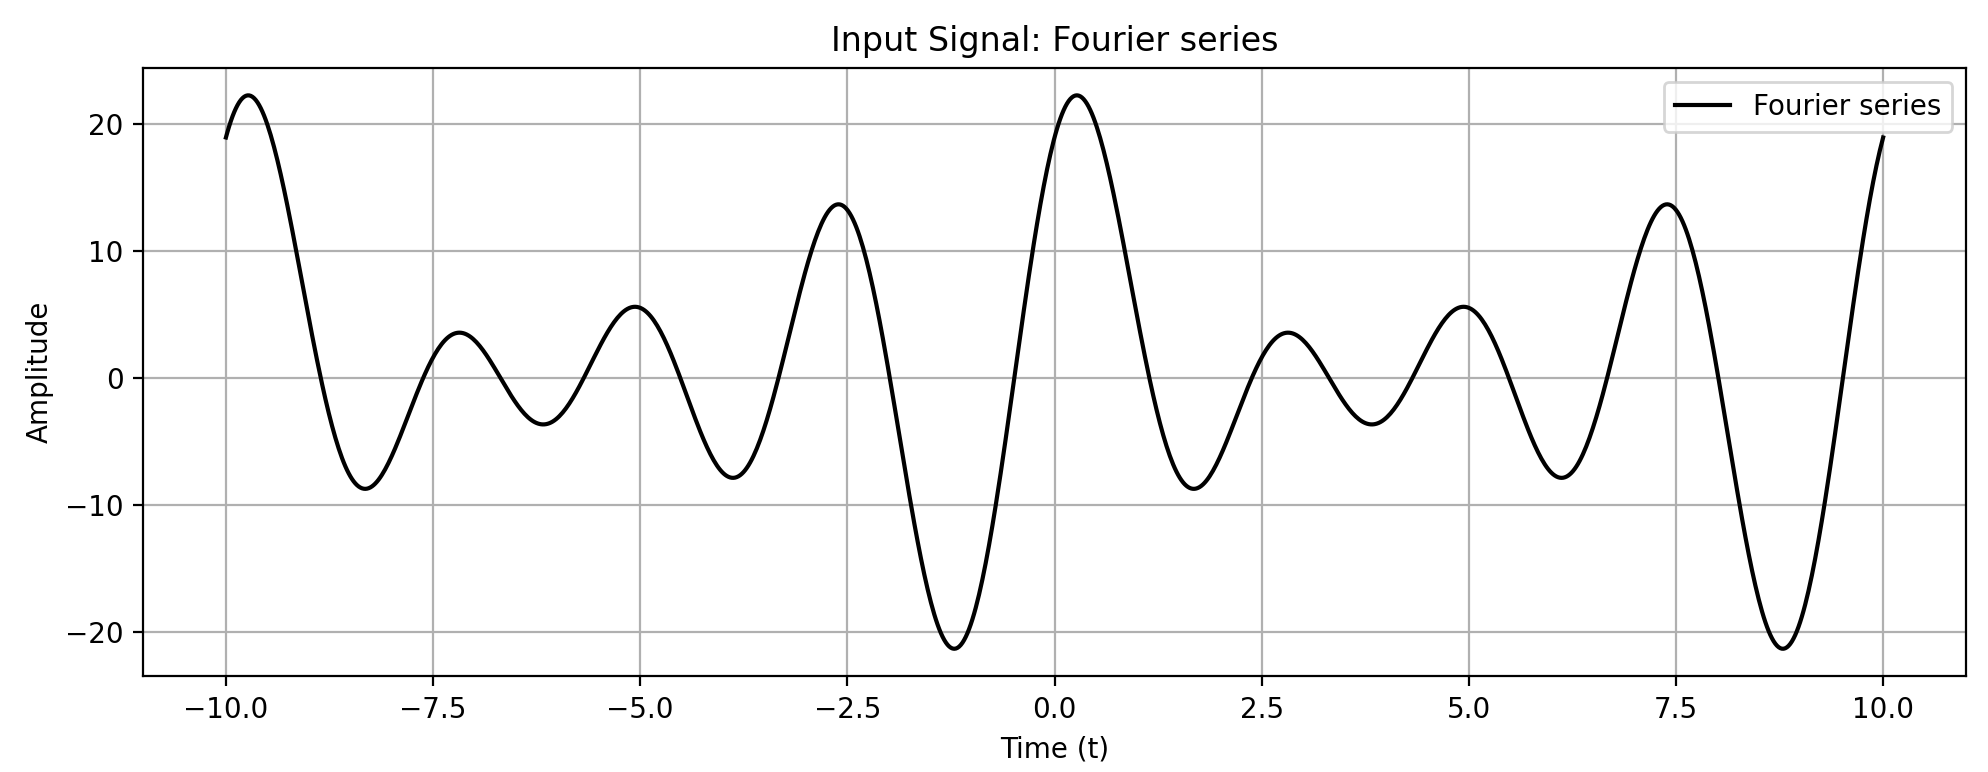
\includegraphics[width=\linewidth]{figs/fourierbreak.png}
\end{figure}
\begin{figure}[H]
    \centering
    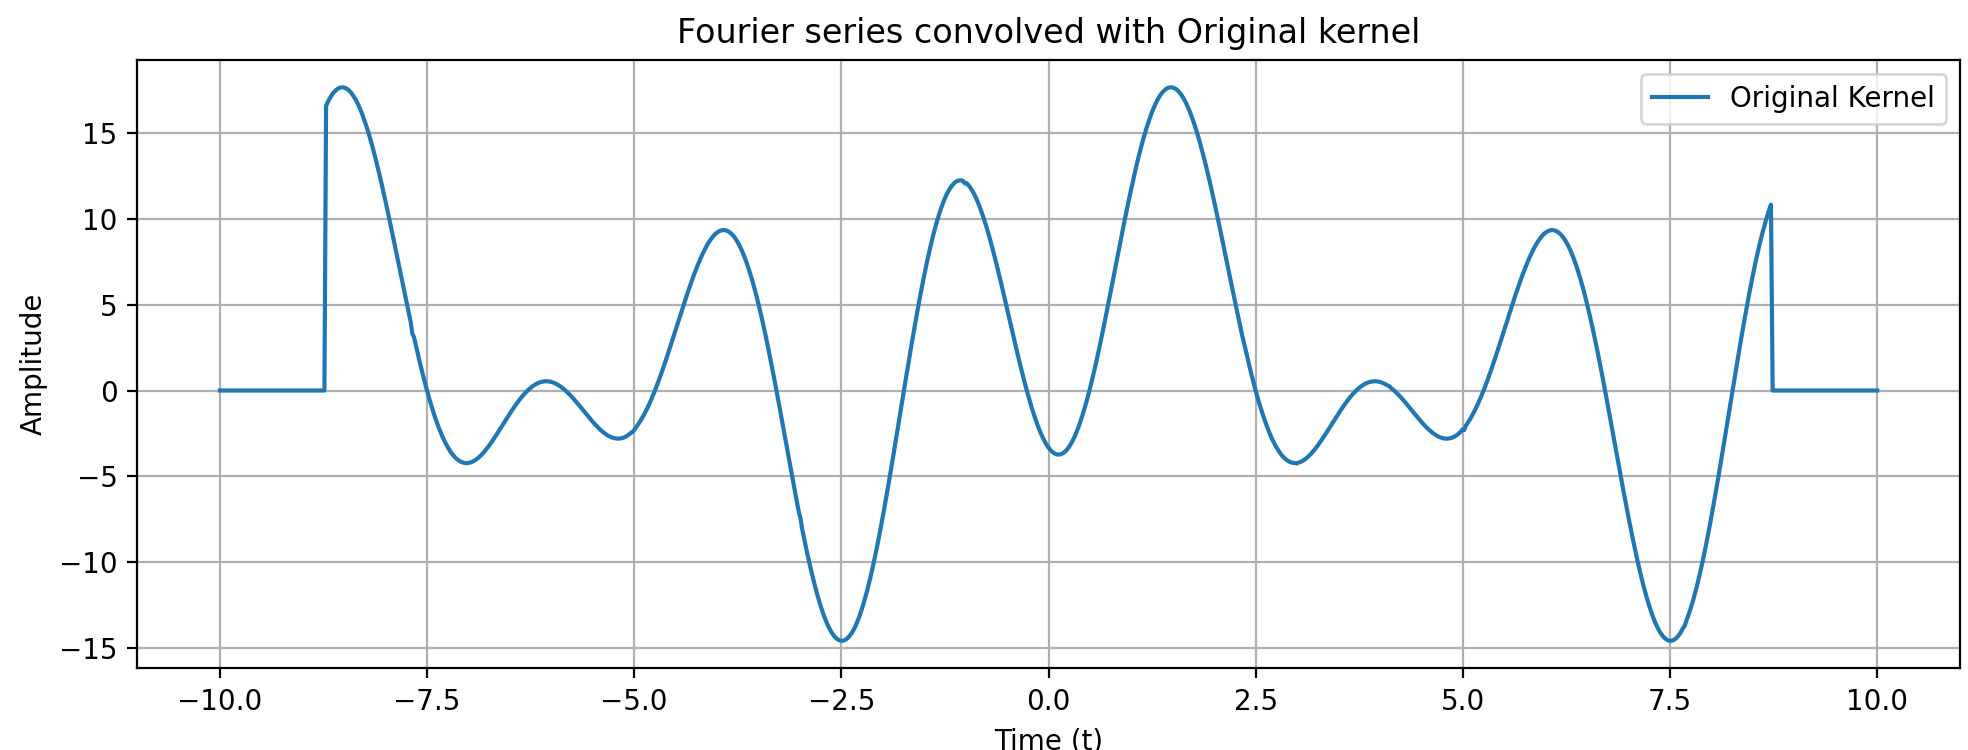
\includegraphics[width=\linewidth]{figs/fourierconv.png}
\end{figure}
\begin{figure}[H]
    \centering
    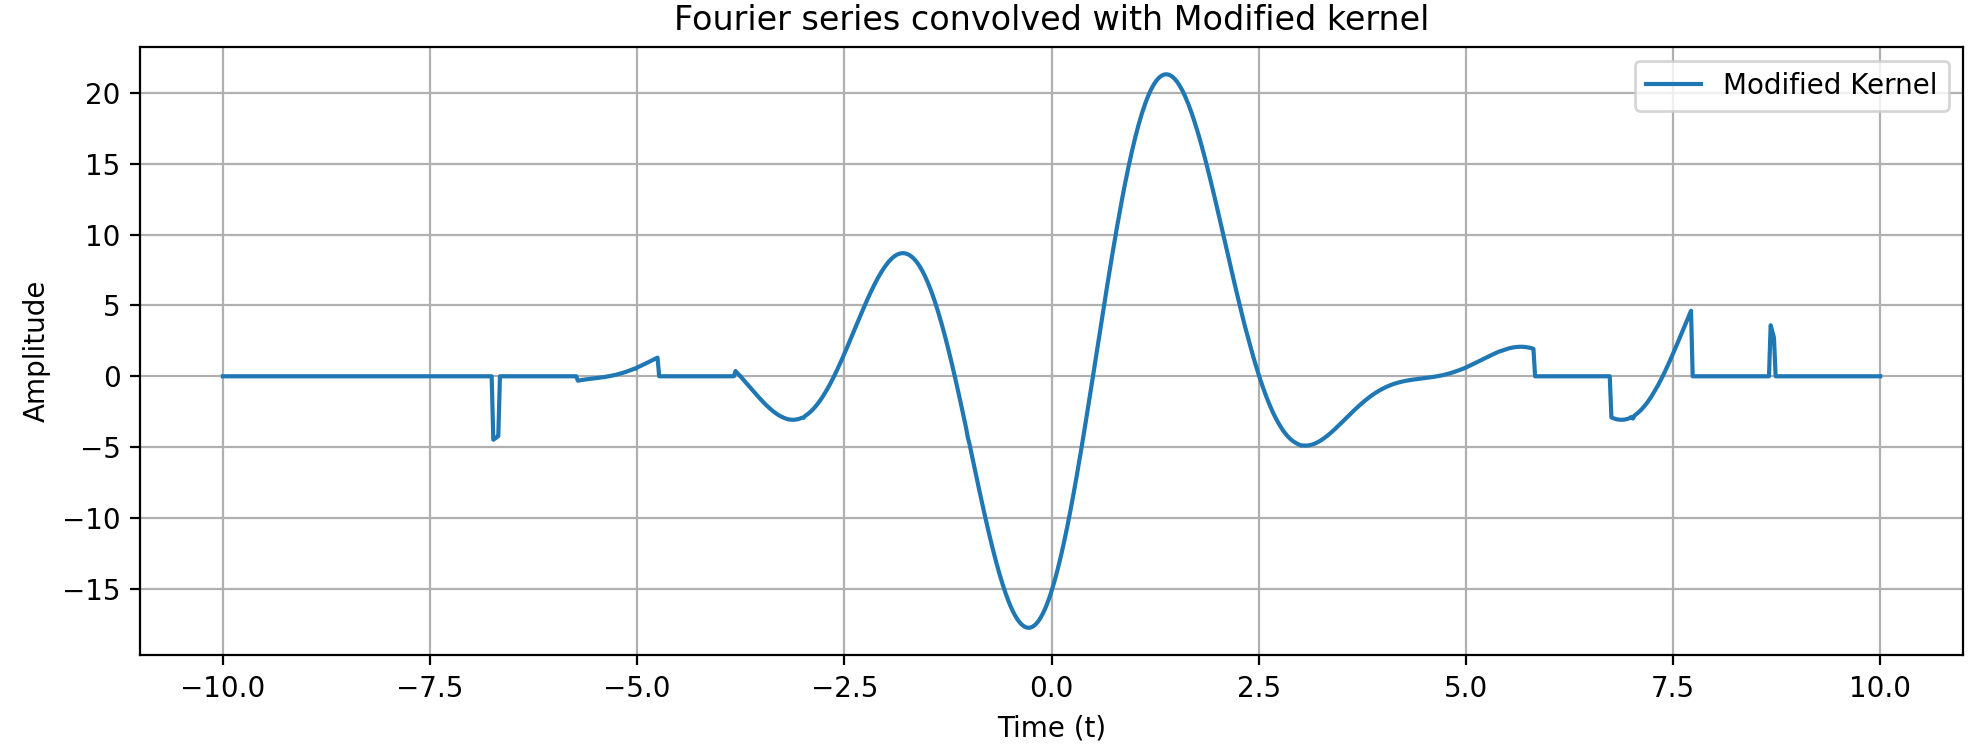
\includegraphics[width=\linewidth]{figs/modifiedfourier.png}
\end{figure}
\begin{figure}[H]
    \centering
    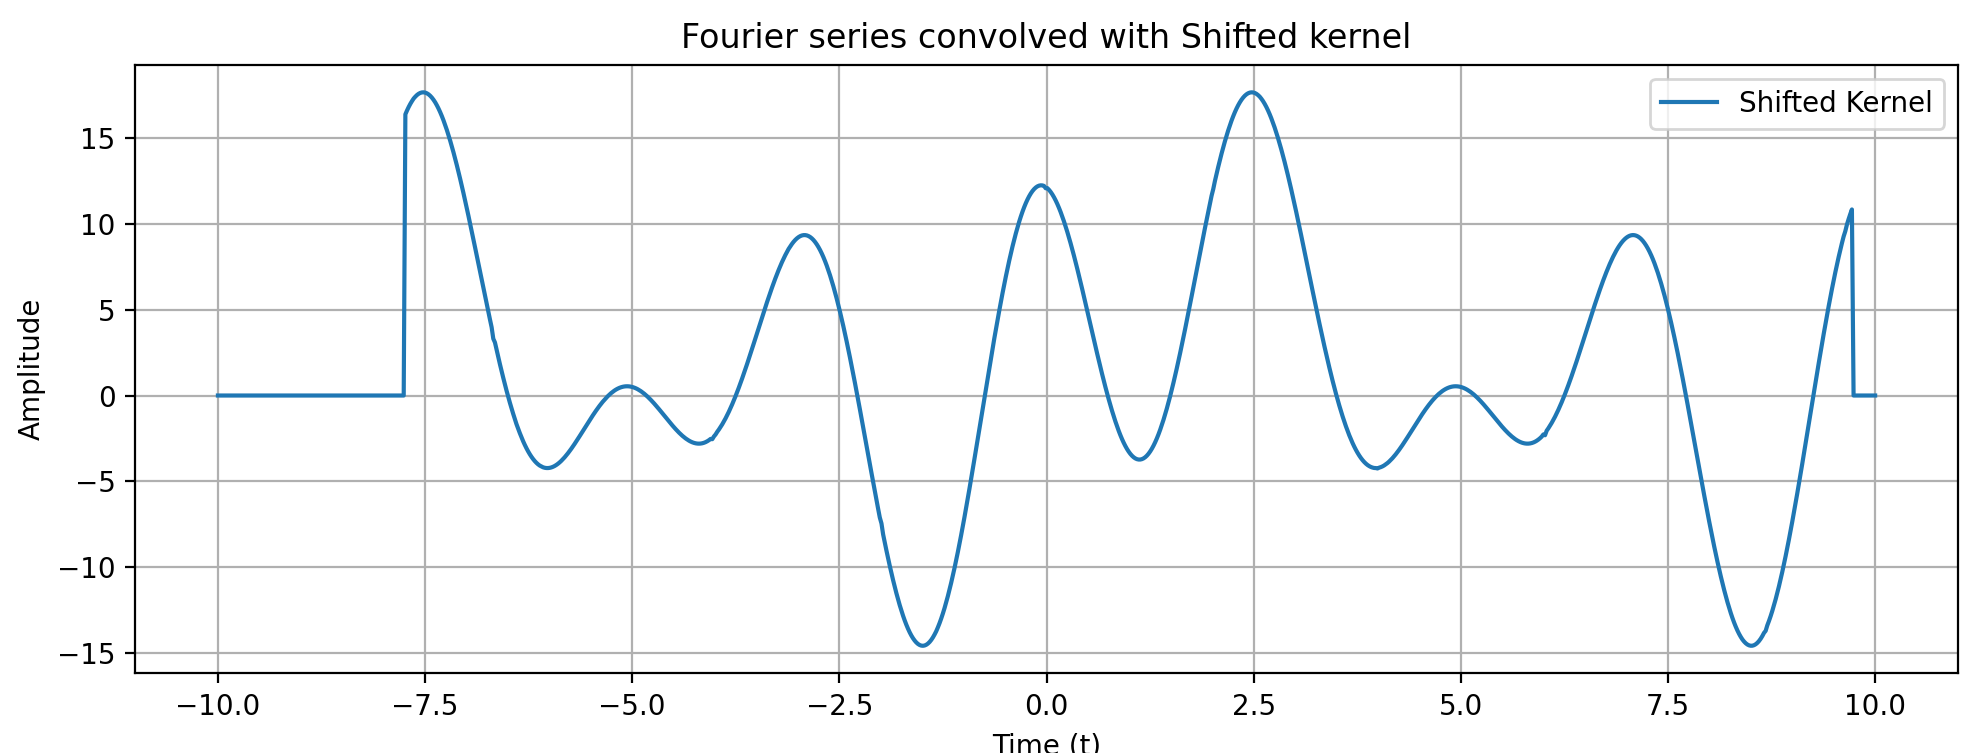
\includegraphics[width=\linewidth]{figs/shiftedfourier.png}
\end{figure}

\end{document}
